\begin{activity} \label{A:2.7.2}  
Consider the curve defined by the equation $y(y^2-1)(y-2) = x(x-1)(x-2)$, whose graph is pictured in Figure~\ref{fig:2.7.Act2}.

Through implicit differentiation, it can be shown that
$$\frac{dy}{dx} = \frac{(x-1)(x-2) + x(x-2) + x(x-1)}{(y^2-1)(y-2) + 2y^2(y-2) + y(y^2-1)}.$$
Use this fact to answer each of the following questions.
\ba
	\item Determine all points $(x,y)$ at which the tangent line to the curve is horizontal.  (Use technology appropriately to find the needed zeros of the relevant polynomial function.)
	\item Determine all points $(x,y)$ at which the tangent line is vertical.  (Use technology appropriately to find the needed zeros of the relevant polynomial function.)
	\item Find the equation of the tangent line to the curve at one of the points where $x = 1$.  
\ea
\end{activity}

\begin{marginfigure}[-5cm]
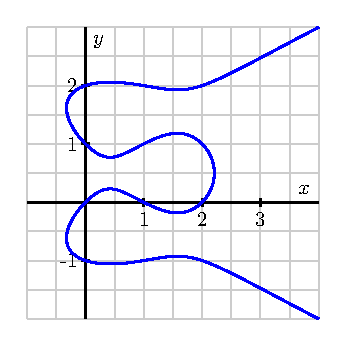
\includegraphics{figures/2_7_Act2.eps}
\caption{The curve $y(y^2-1)(y-2) = x(x-1)(x-2)$.} \label{fig:2.7.Act2}
\end{marginfigure}

\begin{smallhint}
\ba
	\item Note that the numerator of $\frac{dy}{dx}$ is a quadratic function of $x$.
	\item The denominator of $\frac{dy}{dx}$ is a cubic function of $y$.
	\item When $x = 1$, then $y$ must satisfy the equation $y(y^2-1)(y-2) = 0$.
\ea
\end{smallhint}
\begin{bighint}
\ba
	\item Note that the numerator of $\frac{dy}{dx}$ is a quadratic function of $x$.  What are its zeros?
	\item The denominator of $\frac{dy}{dx}$ is a cubic function of $y$.  Use appropriate technology to determine the zeros of this function.
	\item When $x = 1$, then $y$ must satisfy the equation $y(y^2-1)(y-2) = 0$.  Evaluate $\frac{dy}{dx}$ at one such point and use your result appropriately.
\ea
\end{bighint}
\begin{activitySolution}
\ba
	\item To find where the tangent line to the curve is horizontal, we set $\frac{dy}{dx} = 0$, which requires that the numerator be zero, or in other words that
	$$(x-1)(x-2) + x(x-2) + x(x-1) = 0.$$
	Expanding and combining like terms, we find that $3x^2 - 6x + 2 = 0$, which occurs where $x = \frac{3\pm\sqrt{3}}{3} \approx 0.42265, 1.57735$. From the graph in Figure~\ref{F:2.7.Act2}, we observe that at each such $x$-value, there are several corresponding $y$-values for which the tangent line will be horizontal.  For instance, when $x = 0.42265$, then $y$ must satisfy the equation
	$$y(y^2-1)(y-2) = 0.42265(0.42265-1)(0.42265-2) = 0.384900.$$
	Because this is a quartic equation (degree 4) equation in $y$, we use computational technology to help us find the solutions.  Doing so, we find four approximate values for $y$, $y \approx -1.05782, 0.229478, 0.770522, 2.05782$, and thus our estimates for four points at which the tangent line is horizontal are
	$$(0.42265, -1.05782); (0.42265, 0.229478);  (0.42265, 0.770522); (0.42265, 2.05782).$$
	Similar work can be done to find the four points at which the tangent line is horizontal when $x \approx 1.57735$.
	\item The tangent line to the curve is vertical wherever $\frac{dy}{dx}$ is undefined, which occurs precisely where 
	$$(y^2-1)(y-2) + 2y^2(y-2) + y(y^2-1) = 0.$$
	Expanding and combining like terms, we see that we need to solve the cubic equation $4y^3 - 6y^2 - 2y + 2 = 0$; using a computer algebra system, we find that this occurs when $y = \frac{1}{2}, \frac{1 \pm \sqrt{5}}{2}.$  It now remains to find the $x$-coordinate that corresponds to each such $y$-value.  For instance, when $y = \frac{1}{2}$, $x$ must satisfy
	$$\frac{1}{2}(\frac{1}{4}-1)(\frac{1}{2}-2) = x(x-1)(x-2),$$
	or in other words, $x^3 - 3x^2 + 2x = \frac{9}{16}.$  Here, too, we use technology to determine that there is only one such $x$, and $x \approx 2.21028$.  Similar work can be done to find the $x$-values that correspond to $y = \frac{1 \pm \sqrt{5}}{2}$.
	\item There are four points on the curve where $x = 1$, which correspond to the $y$-values that satisfy $y(y^2-1)(y-2) = 0$: $(1,0)$, $(1,1)$, $(1,-1)$, $(1,2)$.  We choose the point $(1,1)$ and evaluate $\frac{dy}{dx}$ at this point.  Doing so,
	  $$\left.\frac{dy}{dx} \right|_{(1,1)} = \frac{(1-1)(1-2) + 1(1-2) + 1(1-1)}{(1^2-1)(1-2) + 2\cdot 1^2(1-2) + 1(1^2-1)} = \frac{-1}{-2} = \frac{1}{2}.$$
Thus, the equation of the tangent line to the curve at $(1,1)$ is $y - 1 = \frac{1}{2}(x-1)$.
\ea
\end{activitySolution}
\aftera